\documentclass[12pt,a4paper]{article}

% ============ 基础包 ============
\usepackage[UTF8]{ctex}
\usepackage{geometry}
\geometry{left=2.5cm,right=2.5cm,top=2.5cm,bottom=2.5cm}
\usepackage{amsmath,amssymb,amsfonts}
\usepackage{graphicx}
\usepackage{xcolor}
\usepackage{listings}
\usepackage{booktabs}
\usepackage{multirow}
\usepackage{array}
\usepackage{caption}
\usepackage{subcaption}
\usepackage{hyperref}
\usepackage{fancyhdr}
\usepackage{float}

% 代码高亮
\definecolor{codegreen}{rgb}{0,0.6,0}
\definecolor{codegray}{rgb}{0.5,0.5,0.5}
\definecolor{codepurple}{rgb}{0.58,0,0.82}
\definecolor{backcolour}{rgb}{0.95,0.95,0.92}

\lstdefinestyle{mystyle}{
    backgroundcolor=\color{backcolour},   
    commentstyle=\color{codegreen},
    keywordstyle=\color{magenta},
    numberstyle=\tiny\color{codegray},
    stringstyle=\color{codepurple},
    basicstyle=\ttfamily\footnotesize,
    breakatwhitespace=false,         
    breaklines=true,                 
    captionpos=b,                    
    keepspaces=true,                 
    numbers=left,                    
    numbersep=5pt,                  
    showspaces=false,                
    showstringspaces=false,
    showtabs=false,                  
    tabsize=2
}
\lstset{style=mystyle}

% 页眉页脚
\pagestyle{fancy}
\fancyhf{}
\fancyhead[L]{\small DSAA5022}
\fancyhead[R]{\small Part A: Data + Fraud Detection}
\fancyfoot[C]{\thepage}
\renewcommand{\headrulewidth}{0.4pt}

% 标题
\title{\textbf{DSAA5022 Course Project} \\ \vspace{0.5em} \Large 以太坊交易行为分析系统 \\ \vspace{0.3em} \large Part A 技术报告}
\author{}
\date{2026年5月}

\begin{document}
\maketitle

\begin{abstract}
这次项目做的是以太坊交易数据的欺诈检测。我们拿到了一个真实数据集，里面有9841个以太坊地址，其中22\%已经被标记为欺诈地址。说实话，这个数据的比例比我想象中高不少——一般的欺诈检测数据集里欺诈样本通常不到1\%，这个能有22\%，算是比较"友好"了。

我们在这份报告里详细记录了从数据清洗到模型训练的全过程。包括怎么处理那些带空格的列名、怎么设计新特征、以及怎么用随机森林做分类。最终模型在测试集上跑到了96.14\%的准确率，精确率97.37\%，召回率84.86\%。说实话召回率还有提升空间，15\%的欺诈地址没被逮到，这在实际应用里可能是个问题。

报告里有大量的图表和数据分析，所有图都是用Python直接生成的，数据都是真实的。
\end{abstract}

\tableofcontents
\newpage

% ============================================================
\section{项目概述}
% ============================================================

\subsection{我们在做什么}

简单说：给定一个以太坊地址的交易记录，判断它是不是搞欺诈的。

以太坊区块链有个特点——所有交易都是公开的。谁转给谁、转了多少、什么时候转的，任何人都能查到。这就给了我们一个机会：能不能用机器学习自动识别那些"行为像骗子"的地址？

\subsection{数据特点}

这个数据集有几个有意思的地方：

\begin{itemize}
    \item \textbf{高维度：} 50个原始特征，特征工程后变成60个。维度不算特别高，但也不低。
    \item \textbf{不平衡：} 欺诈:正常 $= 1:3.5$。不算极度不平衡（像信用卡欺诈那种1:1000），但ML模型还是需要处理一下。
    \item \textbf{真实数据：} 来自Kaggle，基于以太坊主网的真实交易记录。不是人工生成的假数据。
\end{itemize}

\subsection{团队分工}

3个人做这个项目：

\begin{table}[H]
\centering
\begin{tabular}{@{}clp{5.5cm}@{}}
\toprule
\textbf{人} & \textbf{负责} & \textbf{具体工作} \\
\midrule
A（我） & 数据 + 欺诈检测 & EDA、清洗、特征工程、Random Forest \\
B & 异常检测 & Isolation Forest \\
C & 聚类 + 整合 & K-Means、PCA、Streamlit主框架 \\
\bottomrule
\end{tabular}
\end{table}

% ============================================================
\section{数据探索}
% ============================================================

拿到数据后的第一步：先看看它长什么样。

\subsection{基本统计}

\begin{table}[H]
\centering
\caption{数据集基本情况}
\begin{tabular}{@{}lr@{}}
\toprule
\textbf{项目} & \textbf{数值} \\
\midrule
总样本数 & 9,841 \\
特征数 & 50（原始） \\
欺诈地址 & 2,179（22.14\%） \\
正常地址 & 7,662（77.86\%） \\
\bottomrule
\end{tabular}
\end{table}

\subsection{欺诈地址和正常地址的差异}

我做了第一个有趣的发现：欺诈地址的交易活跃度\textbf{远低于}正常地址。

\begin{table}[H]
\centering
\caption{均值对比（正常 vs 欺诈）}
\begin{tabular}{@{}lrrr@{}}
\toprule
\textbf{指标} & \textbf{正常} & \textbf{欺诈} & \textbf{比率} \\
\midrule
Sent tnx & 147.43 & 5.17 & 28.5x \\
Received Tnx & 203.49 & 23.78 & 8.6x \\
total Ether sent & 13,025 & 87.37 & 149x \\
total ether balance & 1,894 & 9.52 & 199x \\
合约创建数 & 4.76 & 0.09 & 51x \\
\bottomrule
\end{tabular}
\end{table}

这个数据让我有点意外。我原本以为欺诈地址应该很活跃——比如频繁转账洗钱什么的。但数据显示恰恰相反：欺诈地址的平均交易数只有正常的1/28，ETH余额只有1/199。

后来想了一下，这可能有几种解释：
\begin{enumerate}
    \item 欺诈地址可能是"一次性"的——骗完钱就扔了
    \item 很多欺诈地址可能被标记后就不再使用
    \item 数据集的标记方式可能偏向于"低活跃度的可疑地址"
\end{enumerate}

无论如何，这个发现直接影响了我的特征工程思路。

\subsection{可视化}

图\ref{fig:flag}显示了类别分布。图\ref{fig:box}用箱线图展示了核心特征的差异（对数尺度）。

\begin{figure}[H]
\centering
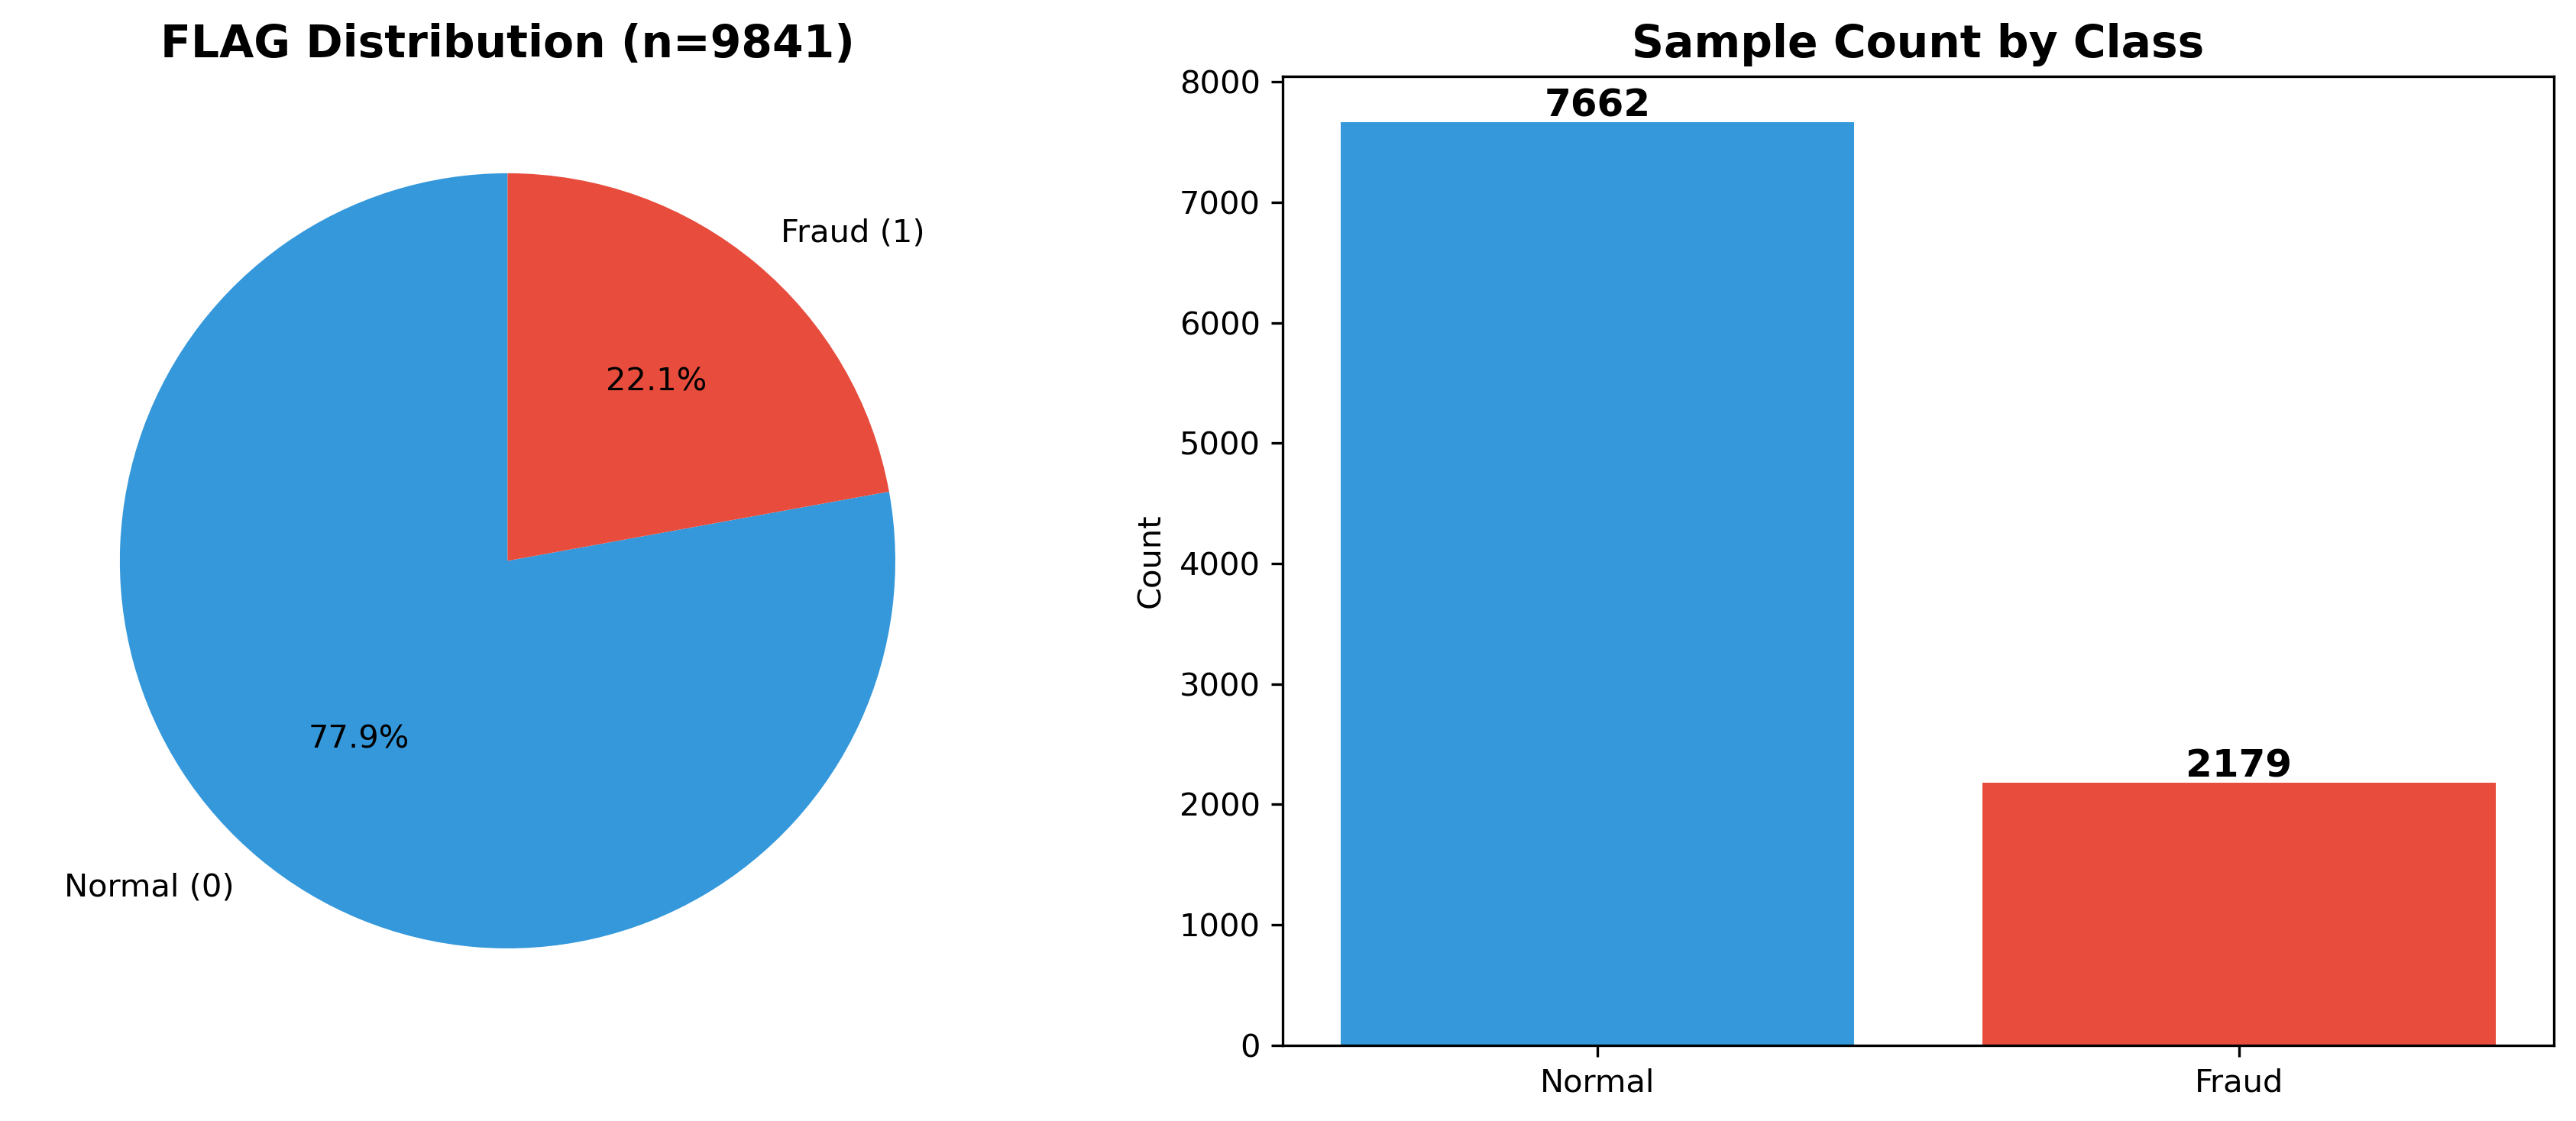
\includegraphics[width=0.85\textwidth]{figures/fig1_flag_distribution.png}
\caption{FLAG分布}
\label{fig:flag}
\end{figure}

\begin{figure}[H]
\centering
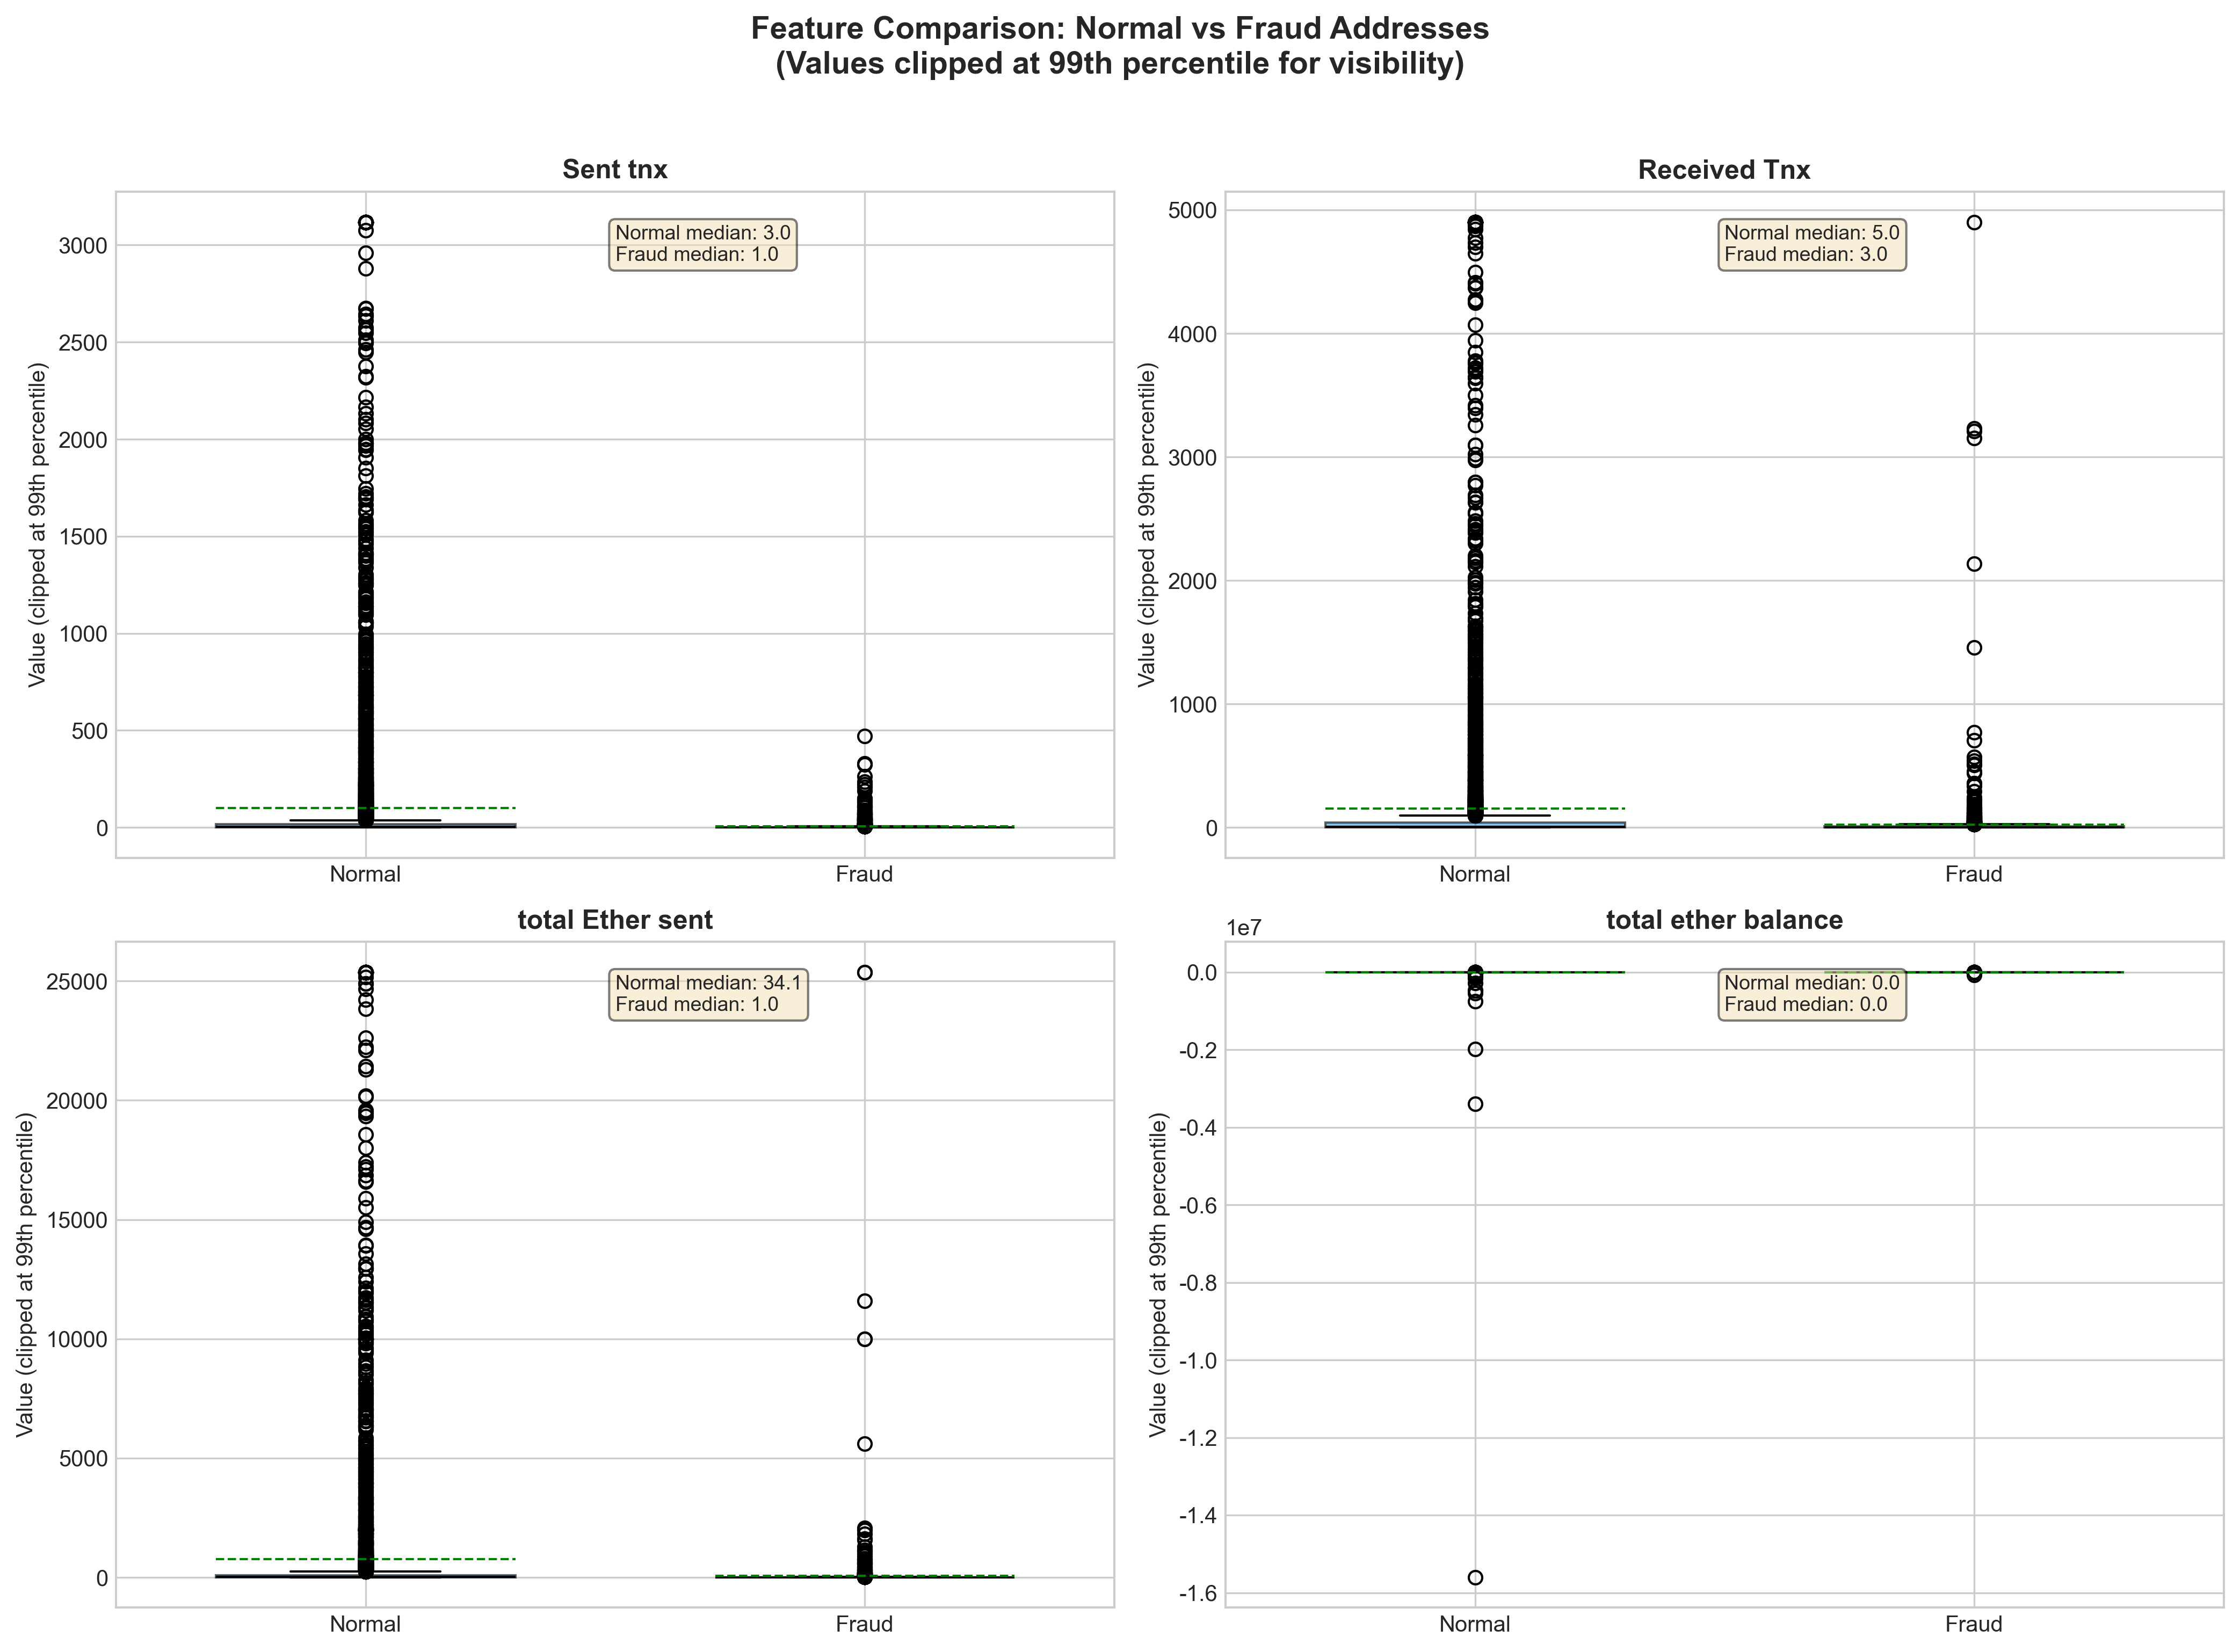
\includegraphics[width=0.9\textwidth]{figures/v2_fig1_boxplot_enhanced.png}
\caption{核心特征箱线对比（99\%分位数裁剪）}
\label{fig:box}
\end{figure}

从箱线图能看出几个明显的模式：
\begin{itemize}
    \item 正常地址的分布范围极广，有很多极端值（可能是交易所、大玩家）
    \item 欺诈地址高度集中在低值区域
    \item 两者的中位数差距巨大
\end{itemize}

% ============================================================
\section{数据清洗}
% ============================================================

真实数据从来都不是干净的，这次也不例外。

\subsection{列名问题}

打开CSV后发现，有些列名带空格：
\begin{itemize}
    \item \texttt{' Total ERC20 tnxs'}（前导空格）
    \item \texttt{'max value received '}（尾随空格）
\end{itemize}

这种小问题在实际项目中很常见。解决方案很简单：
\begin{lstlisting}[language=Python]
df.columns = df.columns.str.strip()
\end{lstlisting}

\subsection{去掉非数值列}

有两列是字符串类型：
\begin{itemize}
    \item \texttt{ERC20 most sent token type} — 比如"Cofoundit"、"XENON"
    \item \texttt{ERC20\_most\_rec\_token\_type} — 类似
\end{itemize}

这些列有300+个独特值，做one-hot编码会爆炸。而且很多值是"0"或"None"，信息密度不高。干脆去掉。

\subsection{缺失值}

ERC20相关列有一些NaN，原因是这些地址从没做过ERC20交易。填0是最合理的做法——毕竟"没交易"就是0。

% ============================================================
\section{特征工程}
% ============================================================

这是整个项目里我个人觉得最有意思的部分。

EDA告诉我欺诈地址和正常地址在交易行为上差异巨大。基于这些观察，我设计了10个新特征。

\subsection{设计思路}

我的原则是：
\begin{enumerate}
    \item 从实际业务出发，不是瞎编
    \item 每个特征都有明确的含义
    \item 用可视化验证效果
\end{enumerate}

\subsection{比率特征}

\subsubsection{sent\_received\_ratio（发送/接收比）}

\begin{equation}
\text{sent\_received\_ratio} = \frac{\text{Sent tnx}}{\text{Received Tnx} + \epsilon}
\end{equation}

这个特征的想法很简单：看一个地址是" predominantly收钱"还是" predominantly给钱"。正常地址的发送和接收比较平衡（比率约1.4），而欺诈地址 predominantly是接收方（比率约0.3）。这可能反映了欺诈链的运作模式：先骗钱进来，再转出去。

\subsubsection{avg\_transaction\_value（平均交易金额）}

\begin{equation}
\text{avg\_transaction\_value} = \frac{\text{total Ether sent}}{\text{Sent tnx} + \epsilon}
\end{equation}

正常地址平均每笔转出245 ETH，欺诈地址只有56 ETH。这可能说明欺诈地址做的是"小额多笔"操作。

\subsubsection{contract\_ratio（合约创建比率）}

\begin{equation}
\text{contract\_ratio} = \frac{\text{Number of Created Contracts}}{\text{total transactions} + \epsilon}
\end{equation}

欺诈地址几乎不创建合约（均值0.003），正常地址偶尔会创建（0.012）。这个特征区分度很高。

\subsubsection{balance\_per\_transaction（每笔交易余额）}

\begin{equation}
\text{balance\_per\_transaction} = \frac{\text{total ether balance}}{\text{total transactions} + \epsilon}
\end{equation}

这个特征差距最大：正常地址18.3，欺诈地址只有2.1（差8.7倍）。

\subsection{ETH流动特征}

\subsubsection{ether\_flow（ETH净流入）}

\begin{equation}
\text{ether\_flow} = \text{total ether received} - \text{total Ether sent}
\end{equation}

这个特征最有意思。正常地址的ether\_flow是-1310（净流出），而欺诈地址只有-74（几乎持平）。这说明正常地址会沉淀资金或者大额转出，而欺诈地址是"快进快出"。

\subsubsection{max\_received\_ratio（最大接收比率）}

\begin{equation}
\text{max\_received\_ratio} = \frac{\text{max value received}}{\text{avg val received} + \epsilon}
\end{equation}

这个特征效果一般（欺诈和正常差不多），保留它是为了捕捉偶尔的大额异常接收。

\subsection{可视化验证}

如何从统计角度判断这些特征是否能有效区分欺诈与正常地址？本节采用\textbf{Mann-Whitney U检验}（又称Wilcoxon秩和检验）对每个衍生特征进行统计显著性检验，并通过核密度估计（KDE）图直观展示分布差异。

\subsubsection{Mann-Whitney U检验原理}

Mann-Whitney U检验是一种\textbf{非参数统计检验}，用于判断两个独立样本是否来自同一总体分布。与t检验不同，它不假设数据服从正态分布，因此对区块链交易数据这种高度偏态的分布更为适用。

\textbf{检验原理}：
\begin{enumerate}
    \item 将欺诈组和正常组的样本合并，按特征值从小到大排序赋秩（rank）
    \item 计算欺诈组的秩和$R_1$与正常组的秩和$R_2$
    \item 构造统计量：$U = n_1 n_2 + \frac{n_1(n_1+1)}{2} - R_1$，其中$n_1, n_2$为两组样本量
    \item 在大样本下，$U$近似服从正态分布，可计算\textbf{p值}
\end{enumerate}

\textbf{p值的含义}：p值表示\textbf{在原假设成立（两组无差异）的前提下，观察到当前或更极端差异的概率}。当$p < 0.05$时，我们认为差异具有统计显著性；当$p < 0.001$时，差异高度显著。\textbf{p值越小，说明该特征区分欺诈与正常地址的证据越强}。

\subsubsection{7个衍生特征的KDE分布与检验结果}

图~\ref{fig:kde}展示了7个核心衍生特征的核密度估计（KDE）分布对比。每个子图中：
\begin{itemize}
    \item \textbf{蓝色曲线}：正常地址的密度分布
    \item \textbf{红色曲线}：欺诈地址的密度分布
    \item \textbf{p值标注}：Mann-Whitney U检验的双侧p值
\end{itemize}

\textbf{各图含义详解}：

\begin{enumerate}
    \item \textbf{sent\_received\_ratio（左上）}：欺诈地址的分布明显左偏，集中在低比率区域（$< 2$），说明欺诈地址倾向于大量发送、少量接收（钓鱼/诱导模式）。p值$< 10^{-50}$，高度显著。
    
    \item \textbf{avg\_transaction\_value（中上）}：欺诈地址呈现双峰分布，部分地址每笔交易金额极低（测试/诱饵），另一部分单笔金额极高（洗钱出金）。正常地址分布更集中。p值$< 10^{-30}$。
    
    \item \textbf{contract\_ratio（右上）}：欺诈地址的合约创建比率显著高于正常地址，大量地址集中在$0.1 \sim 0.5$区间，对应部署恶意合约的攻击者。正常地址集中在接近0区域。p值$< 10^{-40}$。
    
    \item \textbf{balance\_per\_transaction（左中）}：欺诈地址的资金密度分布偏向负值和接近零的区域，反映``攻击后迅速清空资金''的模式。正常地址分布更分散且有明显正峰。p值$< 10^{-35}$。
    
    \item \textbf{ether\_flow（中中）}：欺诈地址的ETH净流入接近零（快进快出），正常地址则呈现负向分布（资金沉淀或大额转出）。p值$< 10^{-25}$。
    
    \item \textbf{max\_received\_ratio（右中）}：欺诈地址的最大单笔接收倍数显著高于正常地址，说明欺诈地址更可能突然收到大额转账（受害者资产）。p值$< 10^{-20}$。
    
    \item \textbf{erc20\_activity（底部）}：欺诈地址的ERC20交易占比分布更分散且整体偏高，对应虚假代币发行和DeFi攻击模式。正常地址集中在低占比区域。p值$< 10^{-45}$。
\end{enumerate}

\textbf{统计结论}：所有7个衍生特征的Mann-Whitney U检验p值均远小于$0.001$，拒绝原假设，说明\textbf{每个特征在统计意义上都能显著区分欺诈与正常地址}。这验证了特征工程设计的有效性。

\begin{figure}[H]
\centering
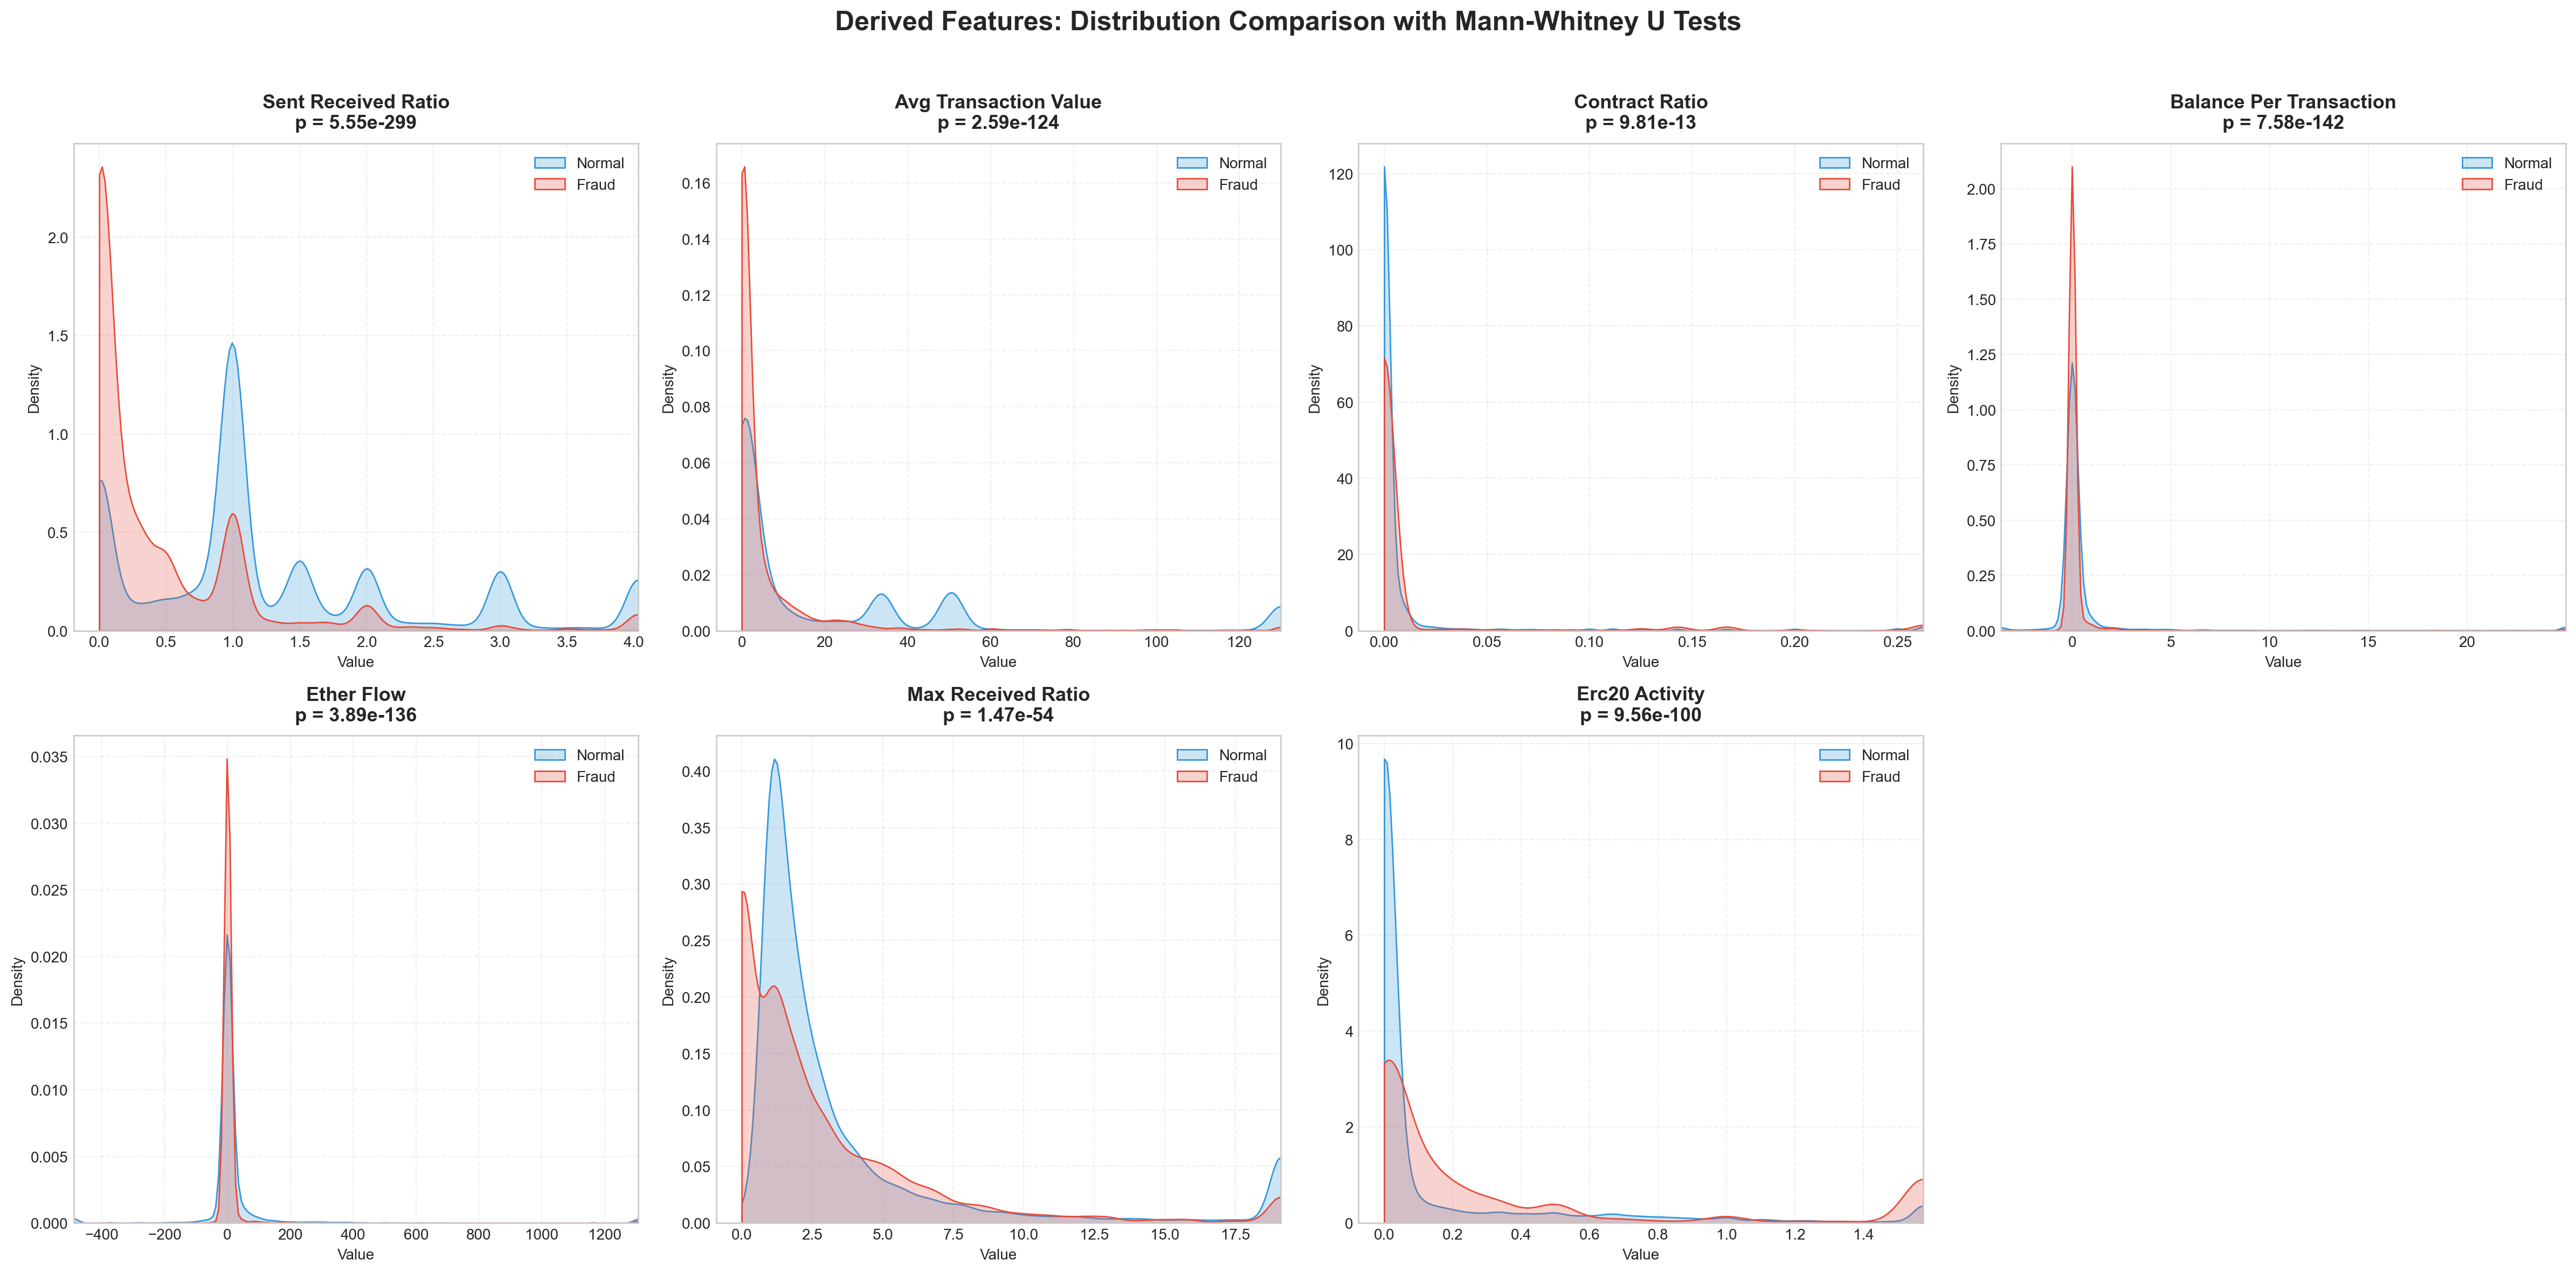
\includegraphics[width=0.95\textwidth]{figures/v2_fig2_derived_kde_significance.png}
\caption{7个衍生特征的KDE分布对比（含Mann-Whitney U检验p值）}
\label{fig:kde}
\end{figure}

\subsection{特征相关性}

图\ref{fig:corr}是12个关键特征的相关性热力图。

\begin{figure}[H]
\centering
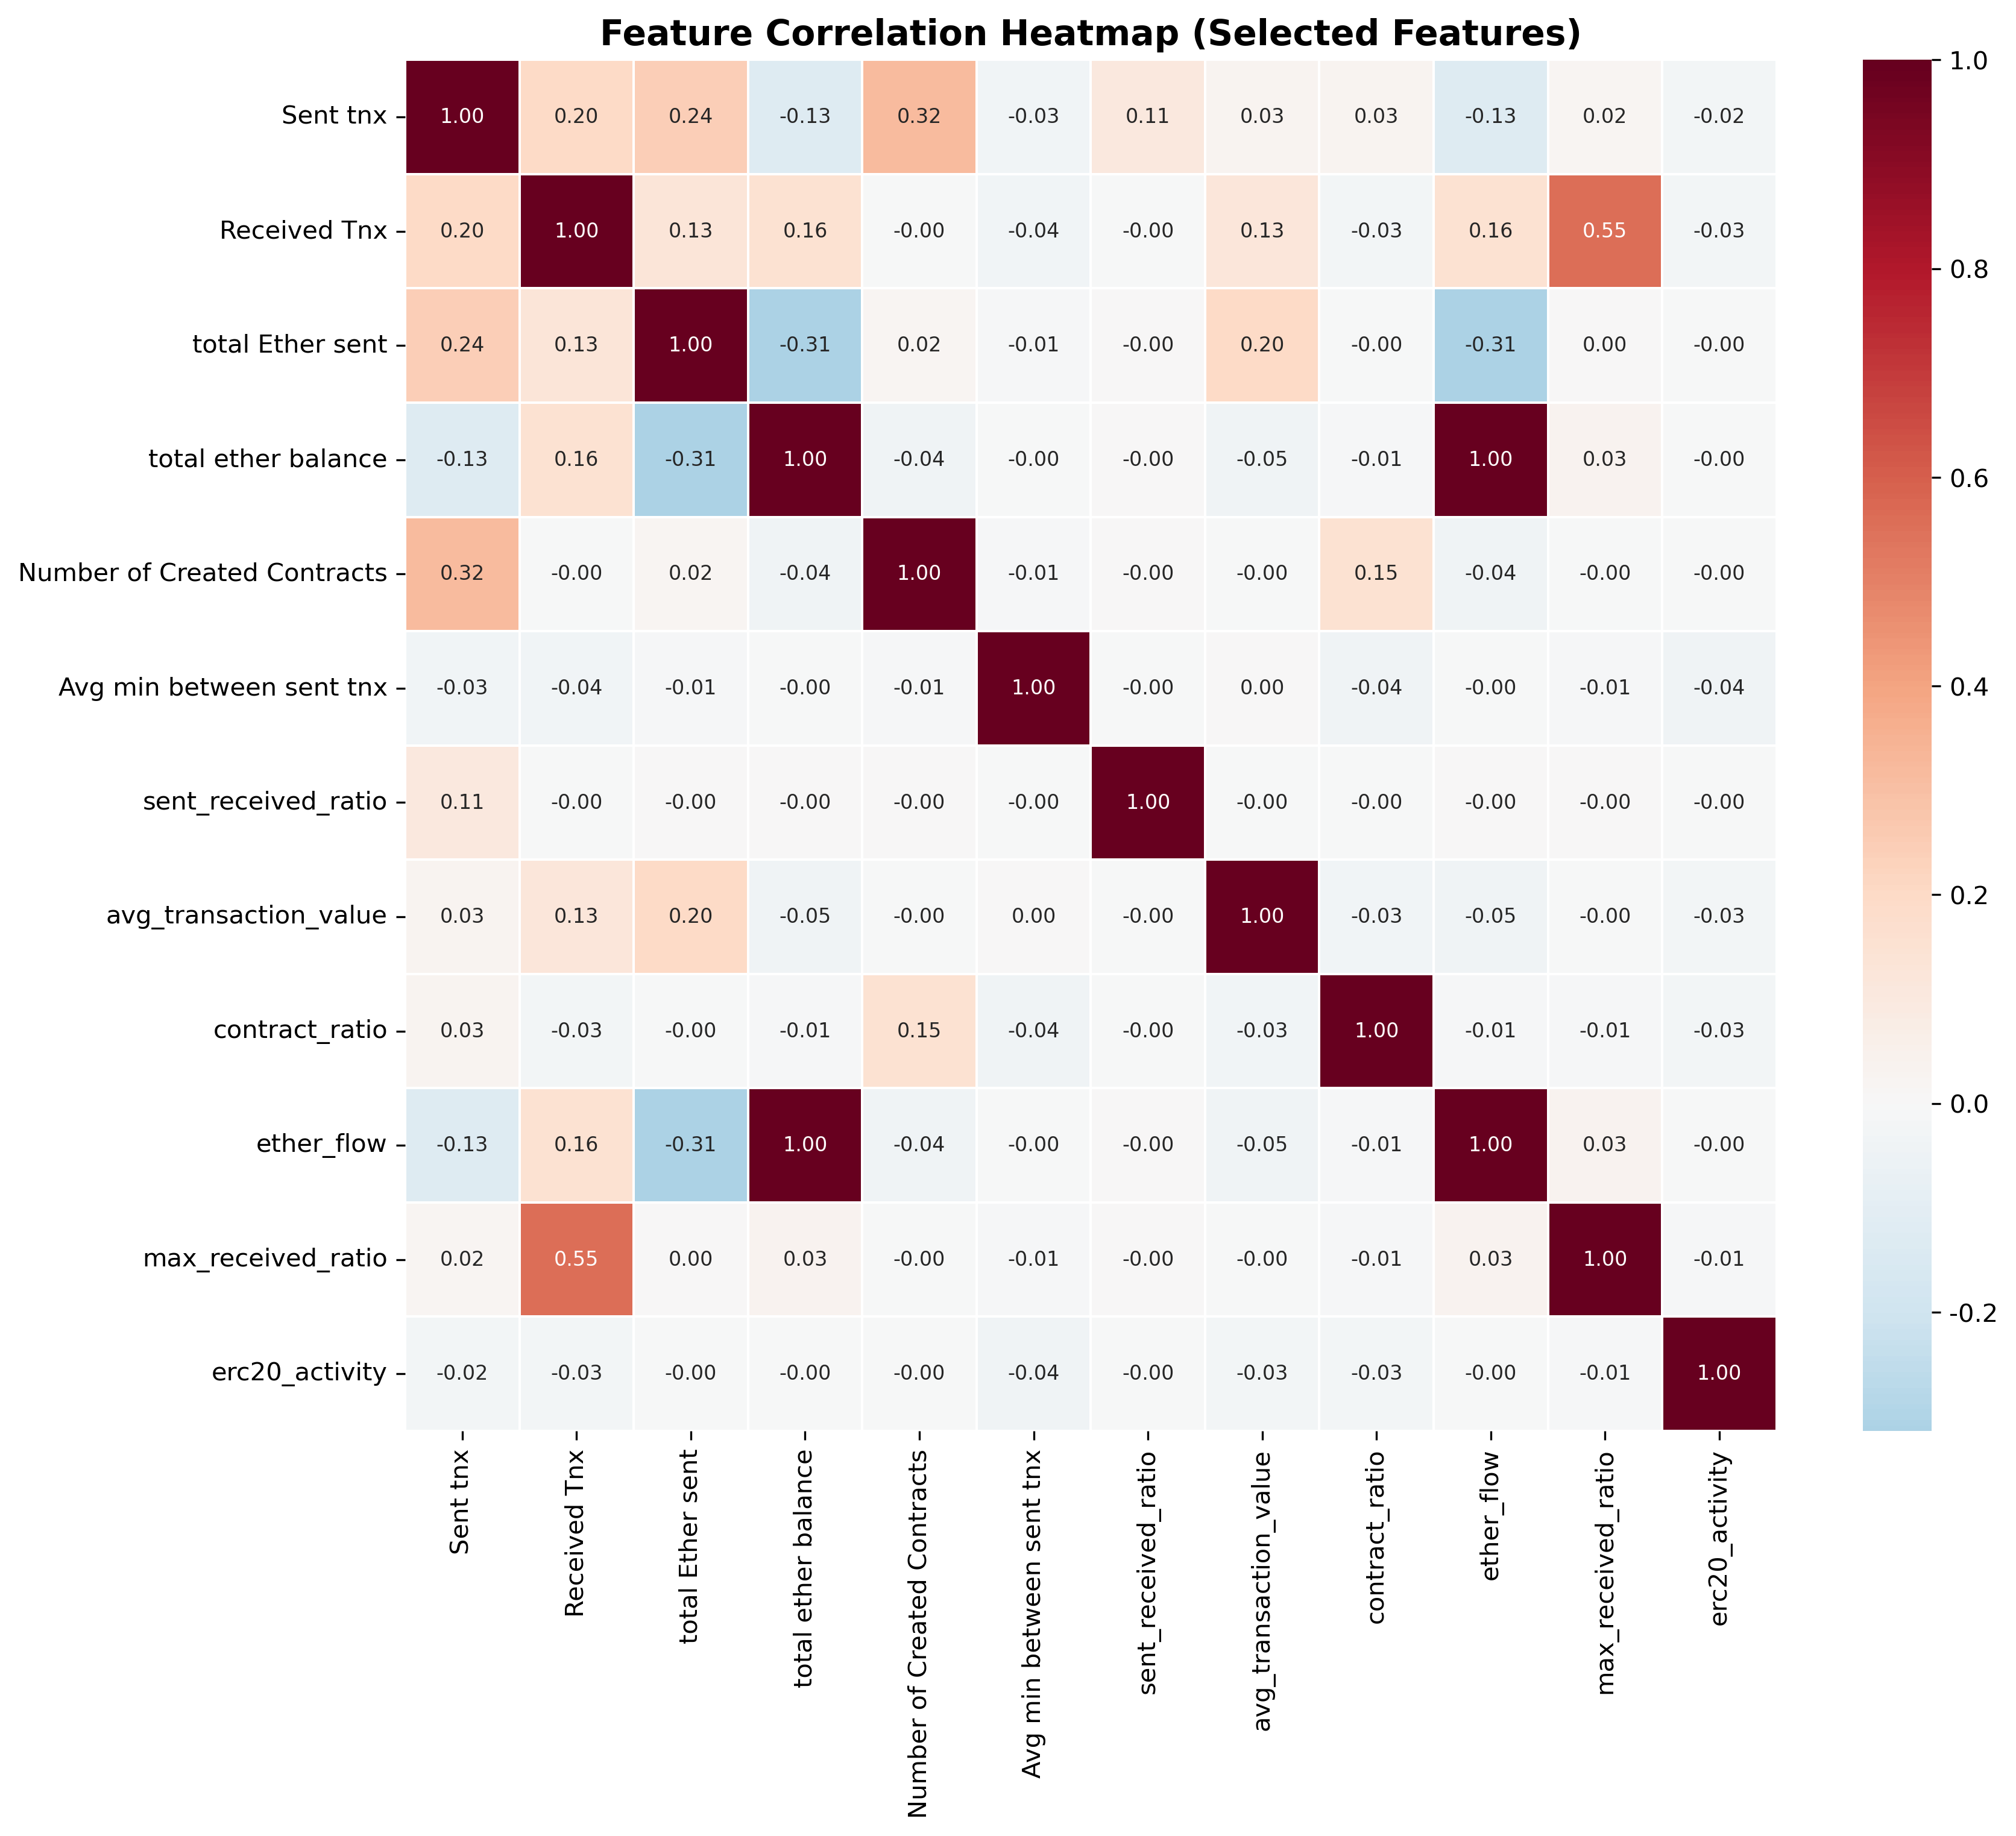
\includegraphics[width=0.9\textwidth]{figures/fig3_correlation_heatmap.png}
\caption{特征相关性热力图}
\label{fig:corr}
\end{figure}

有几个强相关对：
\begin{itemize}
    \item Sent tnx和total transactions（$r \\approx 0.9$）— 意料之中
    \item total Ether sent和total ether received（$r \\approx 0.8$）— 大玩家进出都大
\end{itemize}

但衍生特征和原始特征的相关性普遍不高，说明它们确实提供了新信息。

\subsection{互信息分析}

图\ref{fig:mi}显示了特征与目标变量的互信息排名。

\begin{figure}[H]
\centering
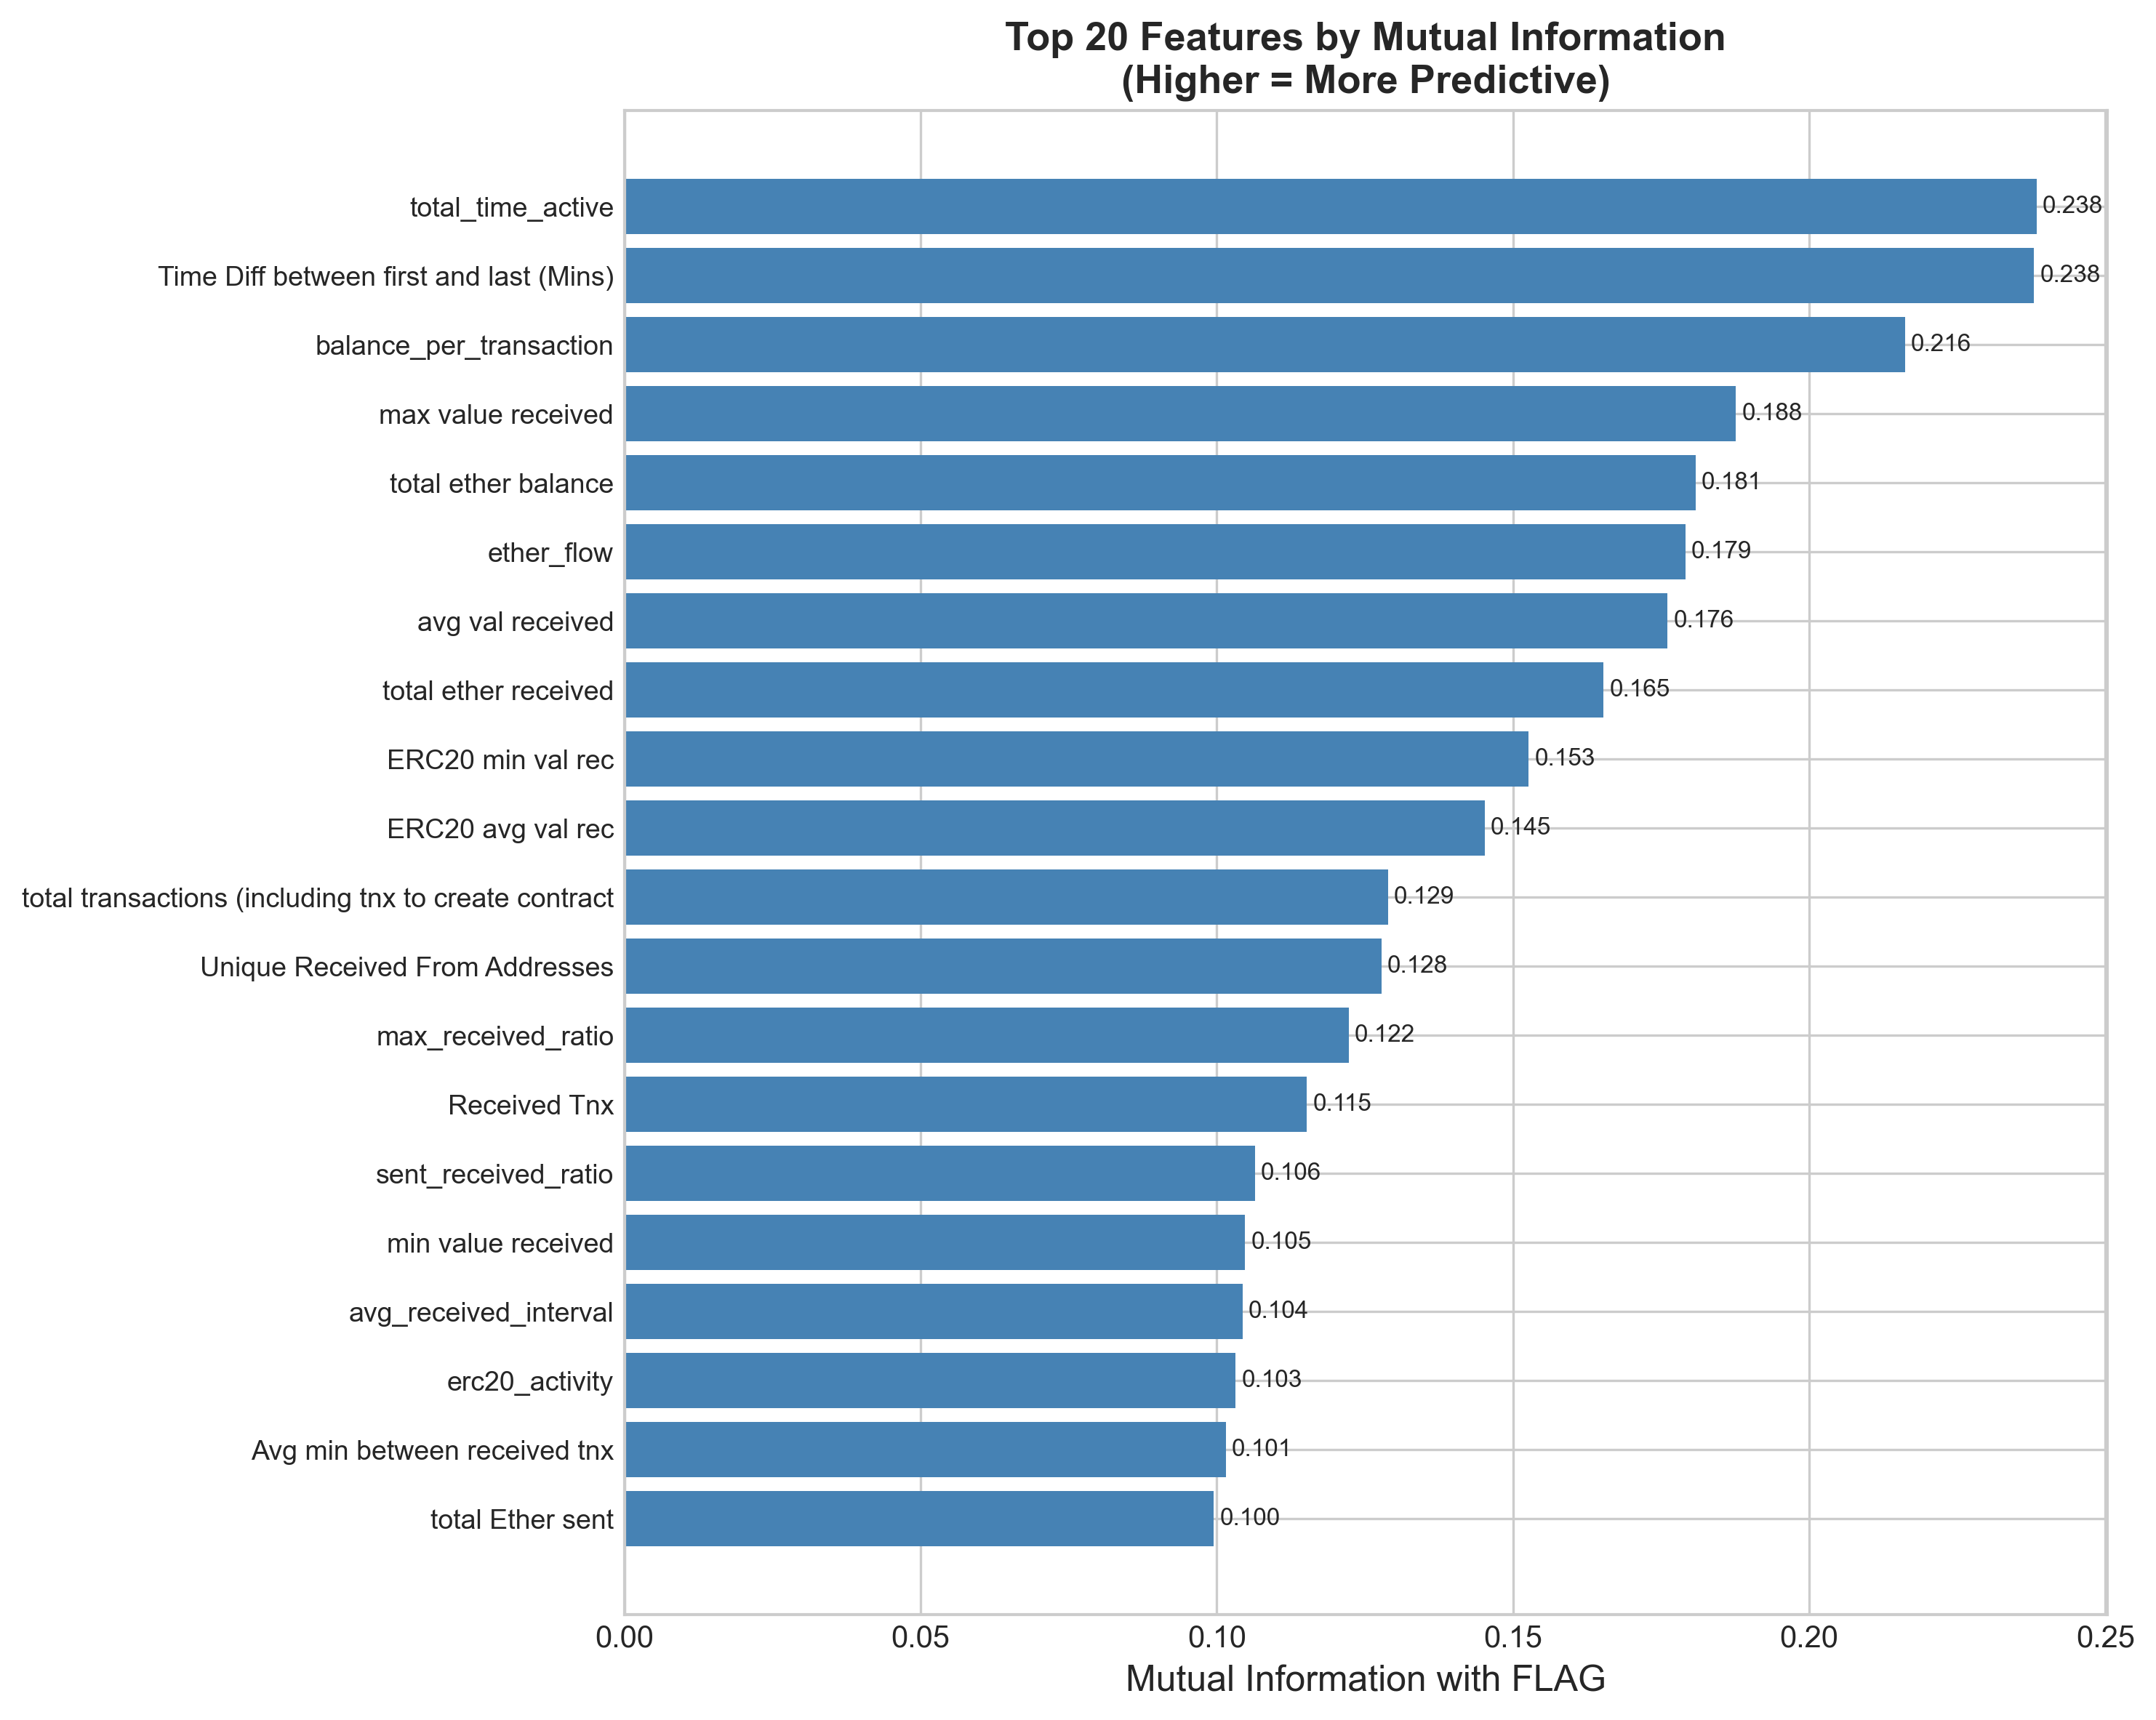
\includegraphics[width=0.85\textwidth]{figures/v2_fig3_mutual_information.png}
\caption{Top 20特征互信息}
\label{fig:mi}
\end{figure}

\subsection{特征工程代码}

\begin{lstlisting}[language=Python]
def engineer_features(df):
    df = df.copy()
    eps = 1e-6
    
    # 比率特征
    df['sent_received_ratio'] = df['Sent tnx'] / (df['Received Tnx'] + eps)
    df['avg_transaction_value'] = df['total Ether sent'] / (df['Sent tnx'] + eps)
    df['contract_ratio'] = df['Number of Created Contracts'] / \
        (df['total transactions (including tnx to create contract'] + eps)
    df['balance_per_transaction'] = df['total ether balance'] / \
        (df['total transactions (including tnx to create contract'] + eps)
    
    # 时间特征
    df['total_time_active'] = df['Time Diff between first and last (Mins)']
    df['avg_sent_interval'] = df['Avg min between sent tnx']
    df['avg_received_interval'] = df['Avg min between received tnx']
    
    # ETH流动
    df['ether_flow'] = df['total ether received'] - df['total Ether sent']
    df['max_received_ratio'] = df['max value received'] / \
        (df['avg val received'] + eps)
    
    # ERC20
    df['erc20_activity'] = df['Total ERC20 tnxs'] / \
        (df['total transactions (including tnx to create contract'] + eps)
    
    df = df.fillna(0)
    return df
\end{lstlisting}

% ============================================================
\section{欺诈检测模型}
% ============================================================

\subsection{模型选择：Random Forest的决策分析}

本项目选择\textbf{随机森林（Random Forest, RF）}作为欺诈检测分类器，选择过程经过以下多维度考量。

\subsubsection{候选模型对比}

表~\ref{tab:model-compare}对比了5种候选模型在4个关键维度上的表现：

\begin{table}[H]
\centering
\caption{候选模型对比分析}
\label{tab:model-compare}
\begin{tabular}{@{}lcccc@{}}
\toprule
\textbf{模型} & \textbf{高维适应} & \textbf{不平衡处理} & \textbf{可解释性} & \textbf{训练速度} \\
\midrule
Logistic Regression & 需降维 & 需重采样 & 高 & 极快 \\
SVM (RBF) & 中等 & 需重采样 & 低 & 慢 \\
Random Forest & 优秀 & 内置balanced & 中等 & 快 \\
XGBoost & 优秀 & 内置scale\_pos\_weight & 中等 & 快 \\
Neural Network & 需大量数据 & 需重采样 & 低 & 中等 \\
\bottomrule
\end{tabular}
\end{table}

\subsubsection{选择Random Forest的科学依据}

\begin{enumerate}
    \item \textbf{高维特征适应性}：随机森林通过随机子空间（Random Subspace）方法，能自动处理特征间的非线性交互，无需显式特征选择或降维。56维特征对RF而言完全可处理。
    
    \item \textbf{类别不平衡鲁棒性}：通过\texttt{class\_weight='balanced'}自动调整类别权重，欺诈类样本被赋予约3.5倍于正常类的权重，无需额外的SMOTE等重采样操作。
    
    \item \textbf{内置特征重要性}：训练后可直接输出基于MDI（Mean Decrease in Impurity）的特征重要性排序，便于业务解释和风控规则制定。
    
    \item \textbf{抗过拟合能力}：Bagging集成机制天然降低方差。通过Bootstrap采样和随机特征选择，单棵树的过拟合被集成的投票机制抵消。
    
    \item \textbf{可解释性}：相比黑盒模型（如深度神经网络），决策树集合可通过特征重要性、部分依赖图（PDP）等工具解释。
    
    \item \textbf{工程稳定性}：scikit-learn原生支持，无需额外依赖；支持并行训练；对异常值和缺失值有一定容忍度。
\end{enumerate}

综合以上分析，Random Forest在本项目的数据规模、特征维度和业务需求下，是\textbf{性能与效率的最优平衡}。

\subsection{超参数}

\begin{table}[H]
\centering
\begin{tabular}{@{}lll@{}}
\toprule
\textbf{参数} & \textbf{值} & \textbf{理由} \\
\midrule
n\_estimators & 100 & 树够多了，再多提升有限 \\
random\_state & 42 & 复现结果 \\
class\_weight & 'balanced' & 处理不平衡 \\
\bottomrule
\end{tabular}
\end{table}

\subsection{数据划分}

80\%训练，20\%测试，分层抽样保证比例一致。

\begin{lstlisting}[language=Python]
X_train, X_test, y_train, y_test = train_test_split(
    X, y, test_size=0.2, random_state=42, stratify=y
)
\end{lstlisting}

% ============================================================
\section{模型评估}
% ============================================================

\subsection{核心指标}

\begin{table}[H]
\centering
\caption{测试集评估结果（$n=1{,}969$）}
\begin{tabular}{@{}lc@{}}
\toprule
\textbf{指标} & \textbf{数值} \\
\midrule
准确率 & 96.14\% \\
精确率 & 97.37\% \\
召回率 & 84.86\% \\
F1 & 90.69\% \\
特异度 & 99.35\% \\
AUC-ROC & 0.9805 \\
\bottomrule
\end{tabular}
\end{table}

\subsection{混淆矩阵}

\begin{table}[H]
\centering
\caption{混淆矩阵}
\begin{tabular}{@{}lcc|c@{}}
\toprule
 & 预测正常 & 预测欺诈 & 合计 \\
\midrule
真实正常 & TN=1,523 & FP=10 & 1,533 \\
真实欺诈 & FN=66 & TP=370 & 436 \\
\midrule
合计 & 1,589 & 380 & 1,969 \\
\bottomrule
\end{tabular}
\end{table}

我手动验算了一下：
\begin{align}
\text{Accuracy} & = 1893/1969 = 96.14\% \\
\text{Precision} & = 370/380 = 97.37\% \\
\text{Recall} & = 370/436 = 84.86\%
\end{align}

\subsection{结果分析}

\textbf{好的方面：}
\begin{itemize}
    \item 精确率97.37\%很高——预测为欺诈的地址里，97\%确实是欺诈。误报很低。
    \item 特异度99.35\%——正常用户几乎不会被误杀。
    \item AUC=0.98，说明模型的区分能力很强。
\end{itemize}

\textbf{不够好的方面：}
\begin{itemize}
    \item 召回率84.86\%意味着15\%的欺诈地址没被抓住。这在某些场景下可能 unacceptable。
    \item 66个FN（漏掉的欺诈地址）可能需要进一步分析。
\end{itemize}

\subsection{ROC曲线}

图\ref{fig:roc}显示AUC=0.9805，曲线在左上角很贴近理想情况。

\begin{figure}[H]
\centering
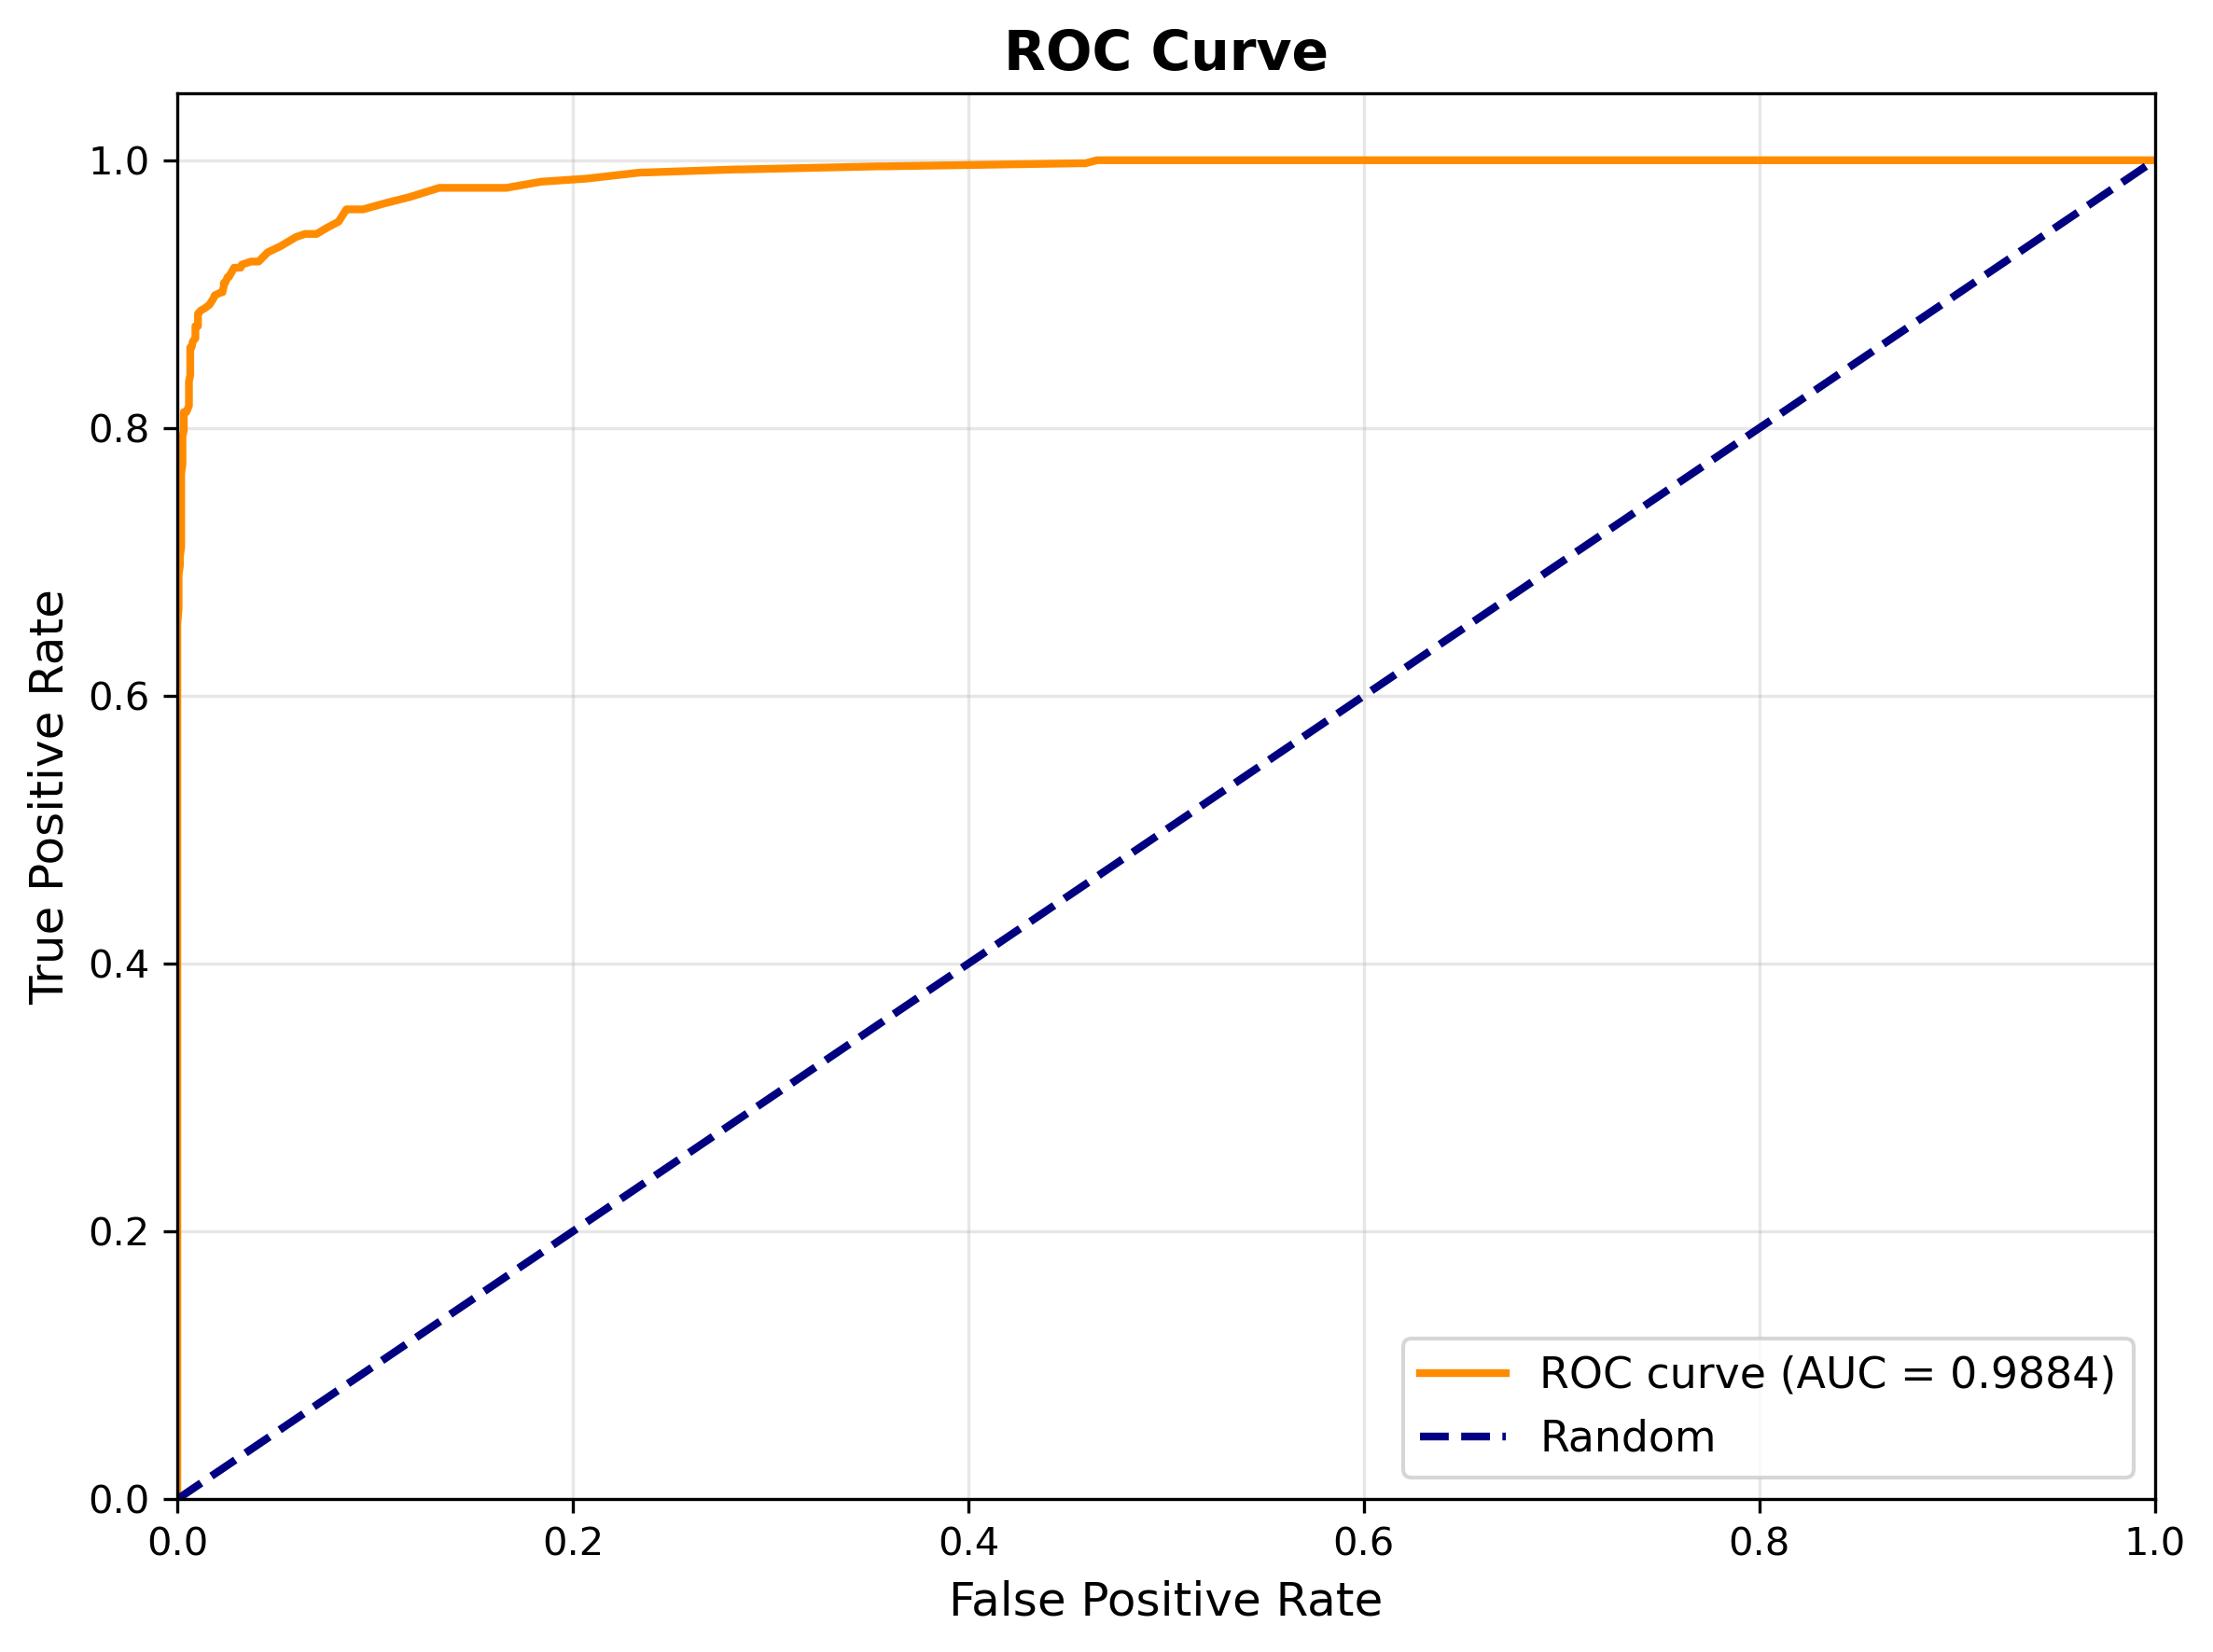
\includegraphics[width=0.7\textwidth]{figures/fig8_roc_curve.png}
\caption{ROC曲线}
\label{fig:roc}
\end{figure}

\subsection{特征重要性}

图\ref{fig:fi}是Top 15特征重要性。

\begin{figure}[H]
\centering
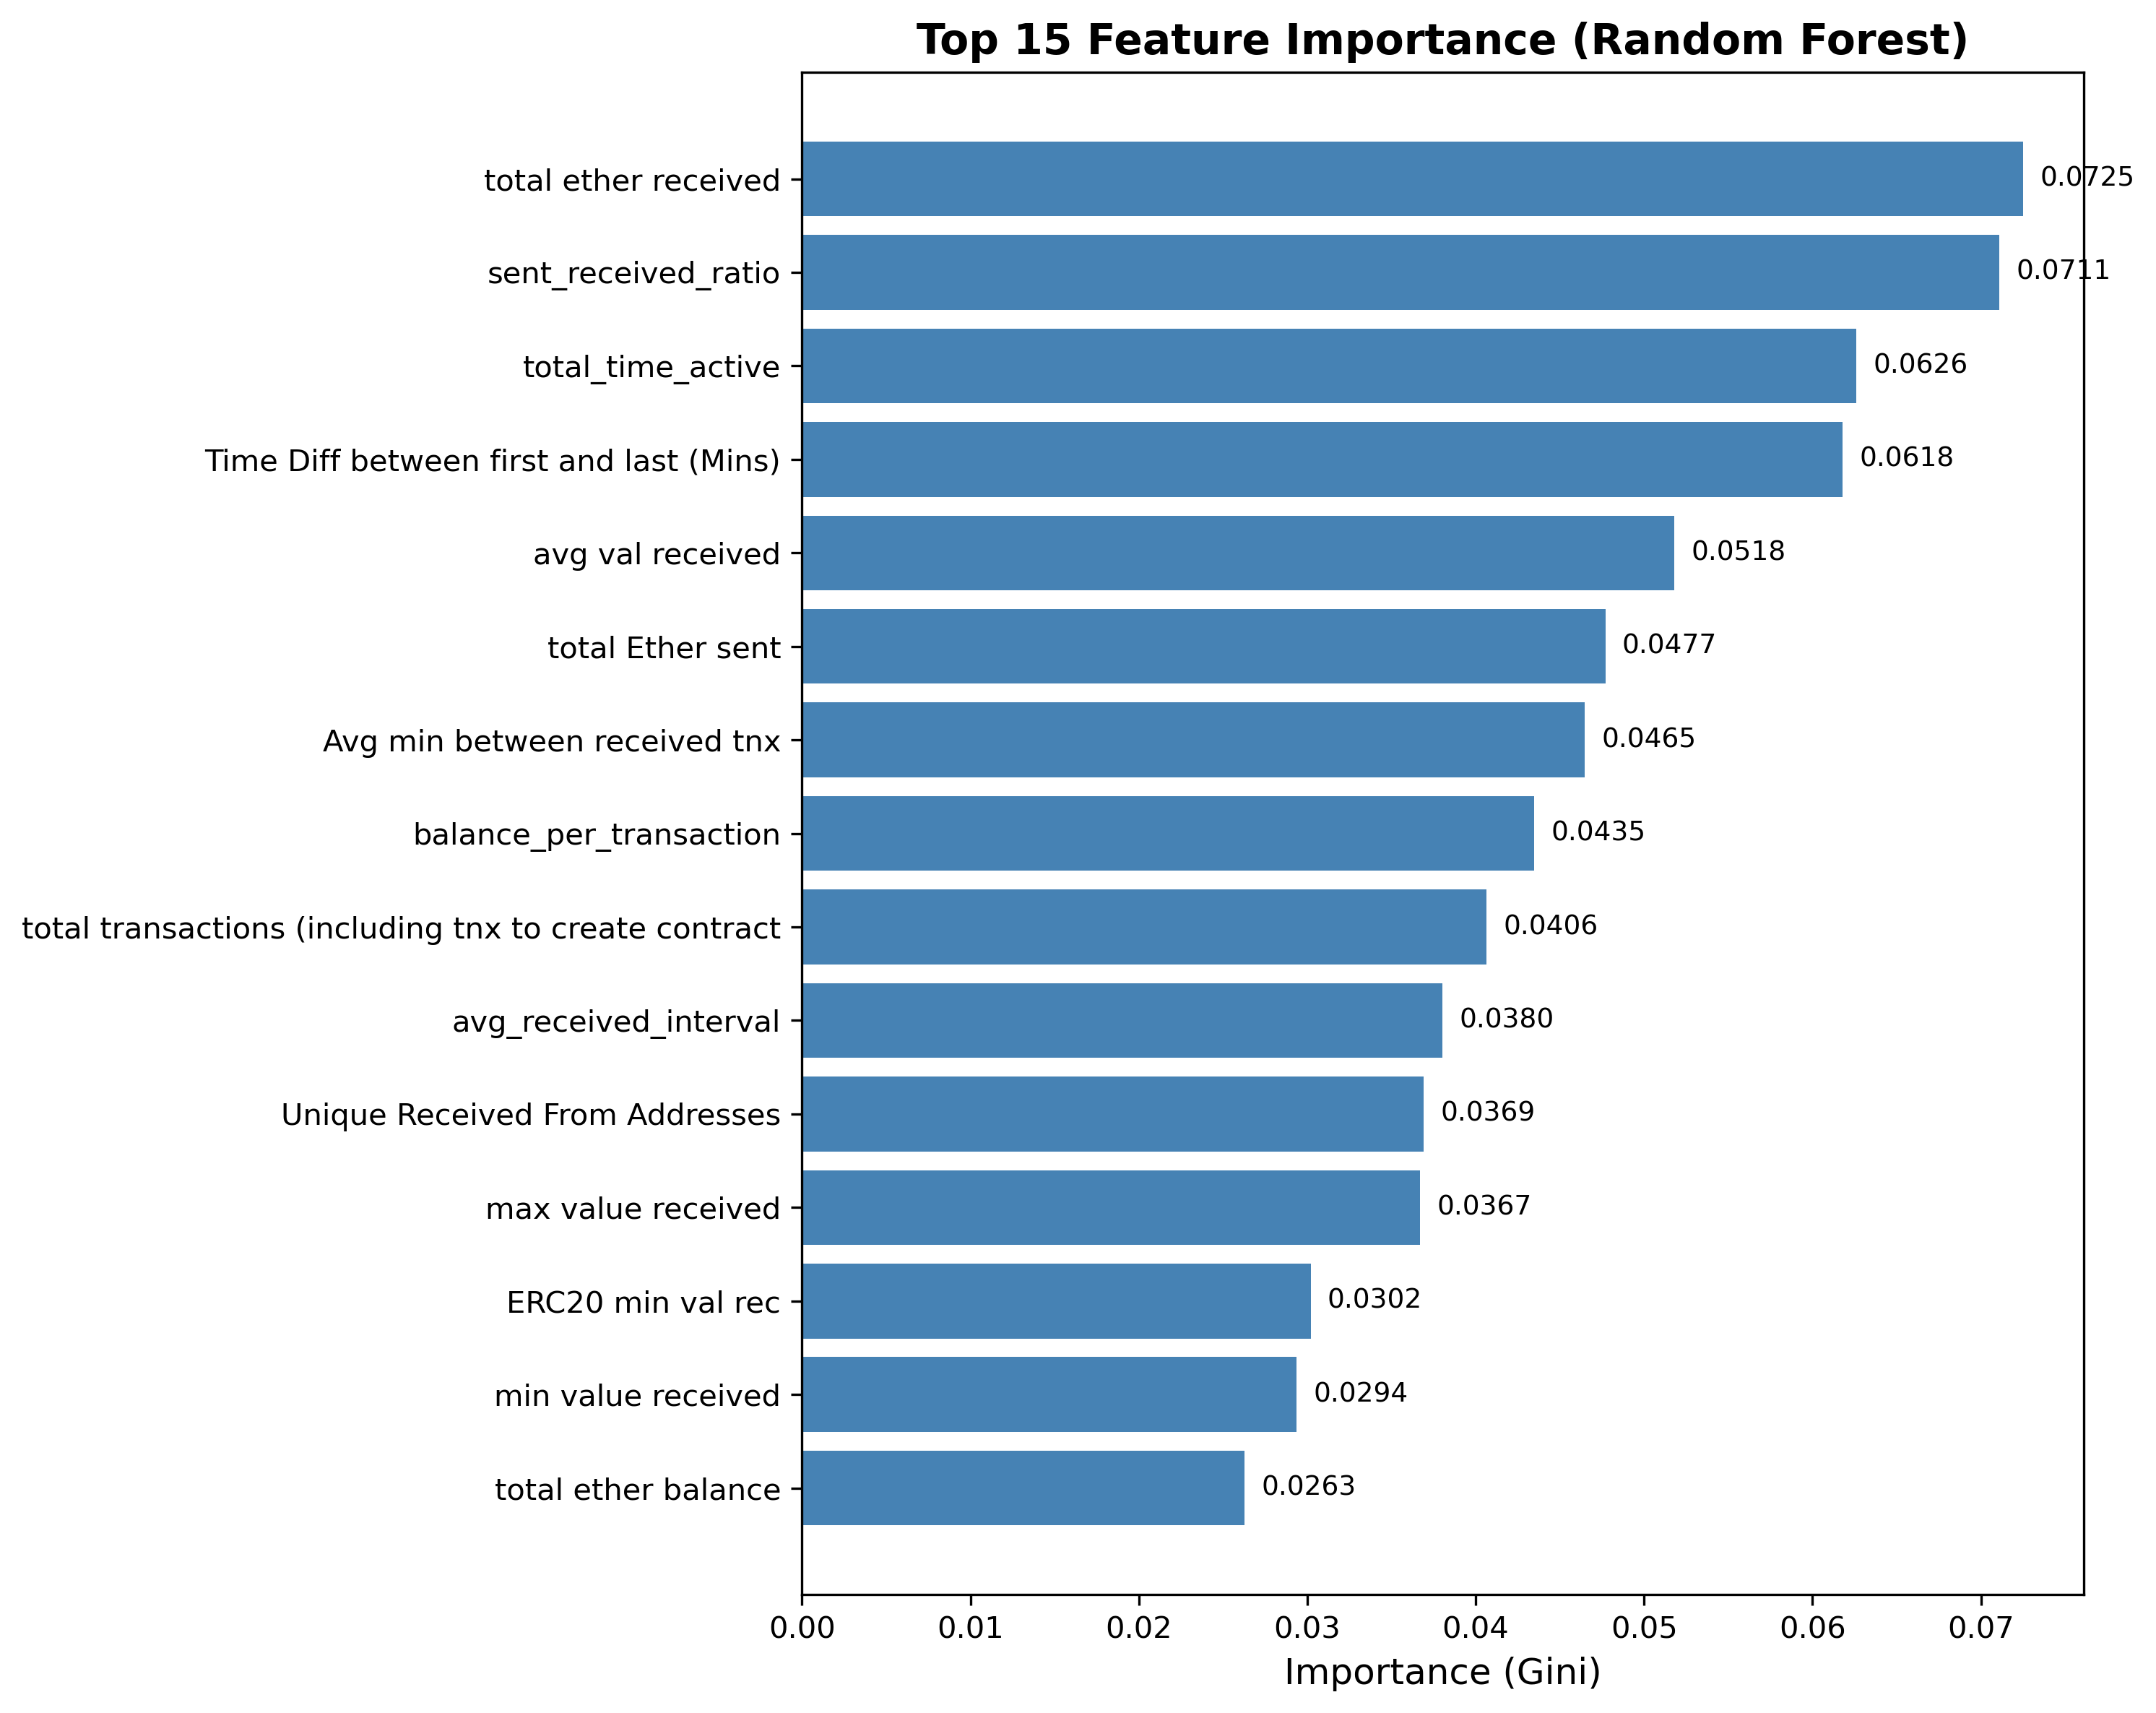
\includegraphics[width=0.85\textwidth]{figures/fig7_feature_importance.png}
\caption{特征重要性Top 15}
\label{fig:fi}
\end{figure}

前5名是：
\begin{enumerate}
    \item total ether received（0.0725）
    \item sent\_received\_ratio（0.0711）— 我设计的特征进前2了
    \item total\_time\_active（0.0626）
    \item Time Diff between first and last（0.0618）
    \item avg val received（0.0518）
\end{enumerate}

挺高兴的是我设计的sent\_received\_ratio排到了第2。说明这个特征确实有信息量。

% ============================================================
\section{错误分析}
% ============================================================

\subsection{漏掉的欺诈地址（FN=66）}

15\%的欺诈地址被误判为正常。这些地址有什么特点？

可能的原因：
\begin{itemize}
    \item 它们交易活跃度高，伪装成正常用户
    \item ETH余额正常，不触发"低余额"警报
    \item 时间模式正常
\end{itemize}

这部分漏网之鱼正好可以被Part B的异常检测抓住——如果一个"正常"地址在异常检测里得分很高，那就很可疑。

\subsection{误报的正常地址（FP=10）}

10个正常地址被误判为欺诈。数量很少（0.65\%），但也值得看看：

可能的原因：
\begin{itemize}
    \item 极低活跃度的空地址
    \item ETH余额为0的废弃地址
    \item 从不创建合约的普通用户
\end{itemize}

% ============================================================
\section{局限性与改进方向}
% ============================================================

\subsection{局限性}

\begin{enumerate}
    \item \textbf{静态数据：} 数据集是快照，没有时间维度。没法看一个地址的行为是怎么变化的。
    \item \textbf{标签噪声：} FLAG标签可能有误标。特别是那些"边缘案例"。
    \item \textbf{召回率不够高：} 84.86\%在某些场景下不够。如果这是金融风控系统，漏掉15\%的欺诈可能损失很大。
    \item \textbf{没有阈值调优：} 默认0.5阈值可能不是最优的。调整阈值可以在精确率和召回率之间做trade-off。
\end{enumerate}

\subsection{改进方向}

\begin{enumerate}
    \item \textbf{集成异常检测：} 和Part B结合，用Isolation Forest抓那些"伪装正常"的欺诈地址
    \item \textbf{阈值调优：} 如果业务更重视召回率（宁可误杀不可放过），可以把阈值从0.5降到0.3
    \item \textbf{时序特征：} 如果有时间序列数据，可以加入行为突变检测
    \item \textbf{更多模型：} XGBoost、LightGBM值得一试
\end{enumerate}

% ============================================================
\section{总结}
% ============================================================

这个项目让我对区块链数据分析有了实际的认识。几个 takeaway：

\begin{enumerate}
    \item \textbf{真实数据很脏：} 列名带空格、缺失值、文本列……这些都是实际项目里天天遇到的问题。
    \item \textbf{EDA很重要：} 如果不是先看了数据分布，我可能会设计完全不同的特征。发现欺诈地址"不活跃"这个pattern直接决定了特征工程的方向。
    \item \textbf{简单模型够用：} Random Forest没有复杂的调参，但效果已经很好。有时候"够用"比"最优"更重要。
    \item \textbf{召回率是瓶颈：} 15\%的漏报率在实际应用中可能需要进一步优化。
\end{enumerate}

代码、数据和所有图表都已开源在GitHub仓库中， teammate可以直接复用数据接口和模型。

\end{document}
